\section{Inspeção em Subestação de Energia Elétrica}

As subestações de energia elétrica representam componentes críticos do sistema elétrico de potência, responsáveis pela transformação, distribuição e controle da energia elétrica. Esta seção apresenta os fundamentos teóricos relacionados às subestações elétricas, métodos de inspeção e aplicações de sistemas robóticos neste contexto.

\subsection{Fundamentos de Subestações Elétricas}
\begin{figure}[h!]
    \centering
%% Figura refeita em 14/11/2026. Na versao anterior o rotulo "Transformador de
%% potencia" aparecia DUAS vezes apontando para objetos diferentes; o rotulo
%% "Barramentos" apontava para uma interligacao em vez do barramento principal; um ramo
%% inteiro ficava sem identificacao; e o para-raios estava em serie na linha, com um
%% aterramento no meio da propria linha principal -- eletricamente, um curto.
    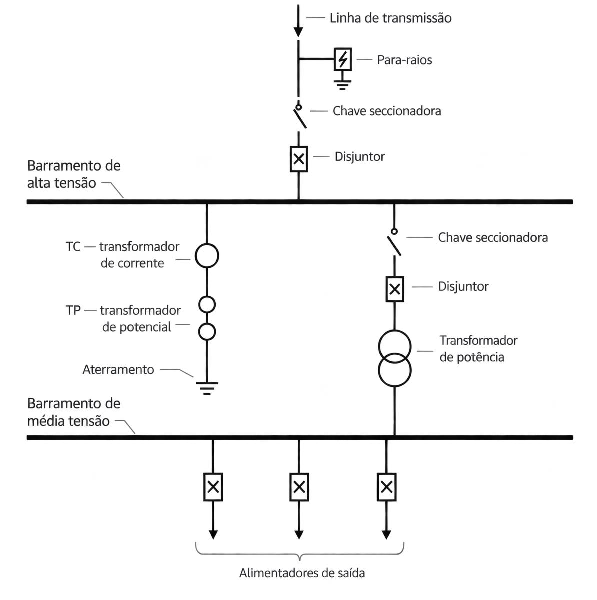
\includegraphics[width=0.8\textwidth]{figuras/fig_subestacao_tipica.pdf}
    \caption{Diagrama unifilar simplificado de uma subestação elétrica típica, da linha
    de transmissão aos alimentadores de saída, com o vão de medição (TC e TP) e o vão de
    transformação derivados do barramento de alta tensão.}
    \legend{Fonte: Adaptado de \citeonline{Muzy2012}.}
    \label{fig:subestacao_tipica}
\end{figure}

Subestações elétricas são instalações que contêm equipamentos para transmissão e distribuição de energia elétrica, além de equipamentos de proteção, medição e controle \cite{Muzy2012}. Elas desempenham funções essenciais no sistema elétrico, incluindo transformação de tensão, seccionamento de linhas, compensação de reativos e interligação de sistemas \cite{Kindermann2012}.

\subsubsection{Classificação e Componentes Principais}

As subestações podem ser classificadas segundo diversos critérios \cite{Mamede2017}:

\begin{itemize}
    \item \textbf{Quanto à função}: Elevadoras, abaixadoras, seccionadoras e de manobra.
    \item \textbf{Quanto ao nível de tensão}: Baixa tensão (até 1 kV), média tensão (1-36,2 kV), alta tensão (36,2-230 kV), extra-alta tensão (acima de 230 kV) e ultra-alta tensão (acima de 800 kV).
    \item \textbf{Quanto ao tipo de instalação}: Convencionais, abrigadas, blindadas, subterrâneas e móveis.
\end{itemize}

Os principais componentes de uma subestação incluem \cite{Frontin2013}:

\begin{itemize}
    \item \textbf{Transformadores de potência}: Responsáveis pela transformação dos níveis de tensão.
    \item \textbf{Equipamentos de manobra}: Disjuntores e chaves seccionadoras.
    \item \textbf{Transformadores de instrumentação}: TCs e TPs para medição e proteção.
    \item \textbf{Equipamentos de proteção}: Para-raios, relés e sistemas de aterramento.
    \item \textbf{Sistemas de controle e supervisão}: SCADA e dispositivos eletrônicos inteligentes (IEDs).
\end{itemize}

O arranjo de barramentos define a configuração física e elétrica da subestação, impactando sua confiabilidade, flexibilidade operativa e custo. Os principais arranjos incluem barra simples, barra principal e transferência, barra dupla, disjuntor e meio, e configuração em anel \cite{Frontin2013}.

\subsection{Normas Técnicas e Regulamentação}

As subestações elétricas são regidas por um conjunto abrangente de normas técnicas e regulamentações que visam garantir a segurança, confiabilidade e padronização das instalações \cite{ABNT2021}. No Brasil, destacam-se as normas ABNT NBR 14039 (média tensão), NBR 5410 (baixa tensão) e NBR 5419 (proteção contra descargas atmosféricas).

Internacionalmente, as normas IEC 61936-1, IEC 62271, IEC 60076 e IEC 61850 estabelecem padrões para instalações de alta tensão, equipamentos de manobra, transformadores e comunicação em subestações, respectivamente \cite{ABNT2021}.

O setor elétrico brasileiro é regulado pela ANEEL (regulação e fiscalização), ONS (operação do sistema), EPE (planejamento) e CCEE (comercialização), com os Procedimentos de Rede do ONS estabelecendo requisitos mínimos para subestações \cite{ONS2020}.

\subsection{Métodos Tradicionais de Inspeção}

A inspeção de subestações elétricas é fundamental para garantir a confiabilidade, segurança e eficiência do sistema elétrico. Tradicionalmente, estas inspeções são realizadas por técnicos especializados, seguindo procedimentos e periodicidades estabelecidos em normas e manuais de manutenção \cite{Silva2019}.

\subsubsection{Principais Métodos}

Os métodos tradicionais de inspeção incluem:

\begin{itemize}
    \item \textbf{Inspeção Visual}: Observação direta dos equipamentos para identificar vazamentos, danos físicos, conexões soltas, trincas em isoladores e outros problemas visíveis \cite{Inovarum2017}.
    
    \item \textbf{Ensaios Elétricos}: Medições de resistência de isolamento, resistência de contato, relação de transformação, fator de potência e testes funcionais de proteção \cite{Conprove2019}.
    
    \item \textbf{Análises Físico-Químicas}: Avaliação de propriedades do óleo isolante, análise de gases dissolvidos e compostos furânicos para equipamentos como transformadores e disjuntores \cite{Inovarum2017}.
    
    \item \textbf{Termografia}: Identificação de pontos de aquecimento anormal através de câmeras termográficas, indicativos de problemas como maus contatos ou sobrecargas \cite{Pixforce2024}.
    
    \item \textbf{Medição de Descargas Parciais}: Detecção de falhas incipientes em isolação elétrica através de métodos acústicos, elétricos ou UHF \cite{Frontin2013}.
\end{itemize}

\subsubsection{Limitações dos Métodos Tradicionais}

Apesar de sua eficácia, os métodos tradicionais apresentam limitações significativas \cite{GlobalGrowthInsights2024}:

\begin{itemize}
    \item \textbf{Exposição a riscos}: Os técnicos estão expostos a riscos elétricos, mecânicos e ambientais.
    \item \textbf{Necessidade de desligamento}: Muitos ensaios requerem o desligamento dos equipamentos.
    \item \textbf{Subjetividade}: A interpretação dos resultados pode variar conforme a experiência do inspetor.
    \item \textbf{Periodicidade limitada}: As inspeções são realizadas em intervalos predefinidos.
    \item \textbf{Custo elevado}: Inspeções manuais requerem mão de obra especializada.
    \item \textbf{Acesso limitado}: Alguns componentes são de difícil acesso para inspeção manual.
\end{itemize}

\subsection{Métodos Avançados e Automatizados de Inspeção}

Para superar as limitações dos métodos tradicionais, têm sido desenvolvidas técnicas avançadas e automatizadas de inspeção, que permitem monitoramento contínuo, maior segurança e detecção precoce de falhas \cite{Wei2024Advancements}.

\subsubsection{Monitoramento Online e Sistemas Integrados}

O monitoramento online permite a avaliação contínua do estado dos equipamentos sem necessidade de desligamento, utilizando sensores para gases dissolvidos em óleo, descargas parciais, temperatura, vibração e sinais acústicos \cite{Clouglobal2024}.

Sistemas de monitoramento integrados combinam diversos sensores e técnicas de análise, frequentemente utilizando comunicação baseada no padrão IEC 61850, que define protocolos e modelos de dados para automação de subestações \cite{Selinc2024}.

\subsubsection{Inspeção por Drones}

O uso de drones para inspeção de subestações oferece vantagens significativas \cite{Pixforce2023}:

\begin{itemize}
    \item Acesso a áreas de difícil alcance
    \item Redução da exposição de técnicos a riscos
    \item Inspeção rápida de grandes áreas
    \item Utilização de múltiplos sensores (visuais, térmicos, UV, LiDAR)
    \item Documentação visual detalhada
\end{itemize}

\subsubsection{Processamento Avançado de Dados}

O volume de dados gerado pelos sistemas de monitoramento e inspeção automatizada requer técnicas avançadas de processamento e análise, incluindo análise de Big Data, inteligência artificial, visão computacional, sistemas especialistas e modelos de Digital Twin \cite{Clouglobal2024}.

\subsection{Robótica para Inspeção de Subestações}

A utilização de robôs para inspeção de subestações representa uma evolução natural dos métodos automatizados, oferecendo vantagens adicionais em termos de segurança, eficiência e capacidade de inspeção \cite{Lactec2022}.

\subsubsection{Tipos de Robôs e Sensores}

Diferentes tipos de robôs têm sido desenvolvidos para inspeção de subestações \cite{GlobalGrowthInsights2024}:

\begin{itemize}
    \item \textbf{Robôs terrestres}: Com rodas, esteiras ou sistemas híbridos de locomoção.
    \item \textbf{Robôs aéreos}: Drones especializados com proteções contra interferência eletromagnética.
    \item \textbf{Robôs escaladores}: Capazes de escalar estruturas verticais.
    \item \textbf{Robôs para linhas energizadas}: Projetados para operar em linhas de transmissão energizadas.
\end{itemize}

Os robôs de inspeção são equipados com diversos sensores \cite{Lactec2022, Iberdrola2022}:

\begin{itemize}
    \item \textbf{Sistemas de visão}: Câmeras RGB, termográficas, UV, estereoscópicas e 360°.
    \item \textbf{Sensores de distância}: LiDAR, ultrassônicos e infravermelhos.
    \item \textbf{Sensores acústicos}: Para detecção de sons anormais, como descargas parciais.
    \item \textbf{Sensores de campo eletromagnético}: Para medição de campos elétricos e magnéticos.
    \item \textbf{Sensores inerciais e de posicionamento}: IMU, GPS/GNSS, RTK e sistemas indoor.
\end{itemize}

\subsubsection{Sistemas de Navegação e Processamento de Dados}

Os sistemas de navegação e controle permitem que os robôs se desloquem de forma segura e eficiente no ambiente da subestação \cite{Lactec2022, Eletrobras2024}, utilizando:

\begin{itemize}
    \item \textbf{Navegação autônoma}: SLAM, planejamento de trajetória e desvio de obstáculos.
    \item \textbf{Controle remoto}: Teleoperação e operação supervisionada.
    \item \textbf{Sistemas de comunicação}: Redes sem fio e comunicação redundante.
\end{itemize}

O processamento dos dados coletados pelos robôs pode ocorrer de forma embarcada (no próprio robô) ou em servidores centrais, utilizando técnicas como visão computacional, aprendizado de máquina e processamento de sinais para identificação de anomalias \cite{Iberdrola2022, Lactec2022}.

\subsection{Casos de Sucesso e Tendências}

Diversos projetos de robótica para inspeção de subestações têm sido implementados com sucesso \cite{Lactec2022, Iberdrola2022}, como:

\begin{itemize}
    \item \textbf{LACBOT}: Robô terrestre autônomo desenvolvido pelo Lactec no Brasil.
    \item \textbf{Antecursor I}: Robô terrestre desenvolvido pela Iberdrola na Espanha.
    \item \textbf{Pix Flight}: Sistema de inspeção baseado em drones desenvolvido no Brasil.
\end{itemize}

As principais tendências na área incluem \cite{GlobalGrowthInsights2024, Wei2024Advancements}:

\begin{itemize}
    \item Maior autonomia dos sistemas robóticos
    \item Utilização de múltiplos robôs cooperativos
    \item Implementação de algoritmos de inteligência artificial mais sofisticados
    \item Integração com modelos digitais (digital twins)
    \item Evolução para robôs capazes de realizar intervenções simples
    \item Implementação de sistemas de recarga autônoma
\end{itemize}

\subsection{Impactos na Manutenção e Operação}

A adoção de sistemas robóticos para inspeção de subestações tem potencial para transformar significativamente as práticas de manutenção e operação \cite{Wei2024Advancements, GlobalGrowthInsights2024}:

\begin{itemize}
    \item \textbf{Evolução para manutenção preditiva}: Intervenções baseadas no estado real dos equipamentos e previsão de falhas.
    \item \textbf{Aumento da confiabilidade}: Detecção precoce de anomalias, redução de falhas inesperadas e extensão da vida útil dos equipamentos.
    \item \textbf{Benefícios econômicos}: Redução de custos operacionais e de perdas por interrupção, apesar do investimento inicial significativo.
    \item \textbf{Segurança do trabalho}: Redução da exposição de trabalhadores a riscos elétricos, trabalho em altura e condições adversas.
\end{itemize}

A inspeção robótica em subestações elétricas representa um campo em rápida evolução, com potencial para superar as limitações dos métodos tradicionais e contribuir significativamente para a modernização e eficiência do setor elétrico.
